\section{Prediction Evaluation}
\label{sec:experiments}

In previous sections, we shown theoretical results with empirical measures  on realization of networks using the generative property of the probabilistic models. In this section, we seek to explain the predictive performance on several datasets by examining their empirical properties and how well the models can capture them. This analysis provide also a study on a comparison of both models, IMMSB and ILFM. Particularly we will see that performance of those models really depend on the type of data we want to fit.

This section is organized as follows:  In first subsection we described our goodness of fit measure used to evaluate various degree distribution. In the second we present the synthetic and real dataset that we have used. In the third we present our prediction evaluation setting. In the last we report our results.

\subsection{A measures for the preferential attachment effect}

\label{sec:experiments-burst}
Preferential attachment leads to networks characterized by a degree distribution with heavy tail. A typical form of such law, often meet in data, is a a power law distribution. Comparison of the degree distribution with a linear function in the log-log scale  gives us a qualitative measure for the preferential attachment. However, for a better evaluation of the power law hypothesis on the degree distribution, we rely on a  goodness a fit based on a Kolmogorov-Smirnov (KS) test. We follow the protocol described in \cite{clauset2009power} which consists of the following steps:
\begin{itemize}
	\item Estimate the parameters $x_{min}$ and $\alpha$ of the power law model.
	\item Calculate the goodness of fit between synthetic datasets generated with the power law and the data. The resulting $p$-values gives an estimates of the  plausibility of the hypothesis for the data.
\end{itemize}

As mentioned in \cite{clauset2009power} high value of the $p$-value should be considered with caution for at least two reasons. First, there may be other distribution that match the data equally or better. Second, a small number of samples of the data may lead to high p-value and reflect the fact that is hard to rule out an hypothesis in such a case.

\subsection{Datasets}
In our experiments, we consider four artificial networks and two real networks.\\

\textit{Artificial networks}

The artificial networks have been generated with ANC-Generator \cite{largeron2015}. This generator has been chosen because it allows to build attributed graphs with  community structure faithfully following the known properties of real-world networks such as preferential attachment and homophily.
Moreover, by modifying the parameters, these properties can be weakened. Finally, ANC-Generator is available under the terms of the GNU Public License and the        parameters can be shared for experiments reproducibility.

Four artificial networks have been generated, each one corresponding to a configuration  regarding the properties of interest.
Table \ref{table:artificial_networks} summarizes these four configurations. We report the seed and parameters that we use those synthetic networks in appendix \ref{seed_dancer	}. Each generated networks correspond to a different combination where homophily and preferential attachment are more or less characterizing the underlying networks. For example...

\begin{table}[h] \label{table:artificial_networks}
	\caption{Artificial networks characteristic.}
	\begin{tabular}{lrrrr}
		\hline
		Networks   &  p-value    &  Modularity & Clustering coefff & density   \\
		\hline
		$Network1$    & 1 &0.59  & 0.06 & 0.007  \\
		$Network2$   & 1 &0.43  & 0.08 & 0.006\\
		$Network3$  & 0.52  &0.71  & 0.49 & 0.01 \\
		$Network4$   & 0.57  &0.68  & 0.61 & 0.06 \\
		\hline
	\end{tabular}
	\caption{Real networks characteristic}
	\begin{tabular}{lrrrr}
		\hline
		Networks    &  p-value    &  Modularity & Clustering coefff & density   \\
		\hline
		$fb\_uc$          & 1 & -  & 0.10 & 0.008 \\
		$manufacturing$   & 0.42 & -  & 0.59 & 0.24 \\
	\end{tabular}
\end{table}

\textit{Real networks}

We also used two real world networks for our experiments .
The first one \footnote{available at:} is built from an online community of 1899 students from the University of California. Each node corresponds to a user and a    directed edge represents a sent message.
The second one \footnote{available at:} is an internal email communication network between employees of a mid-sized manufacturing company. Each vertex is associated  to an employee and an oriented link represents like previously a sent email.

Table 1 summarizes some properties characteristics of these artificial and real datasets. The  p-value is computed as described in \ref{sec:experiments-burst } as a reference for the global preferential attachment effect. we also report the modularity on the a given (true) partition (by Dancer) of the networks, and the clustering coefficient.

\begin{figure}[h]
	\centering
	
	\minipage{0.25\textwidth}
	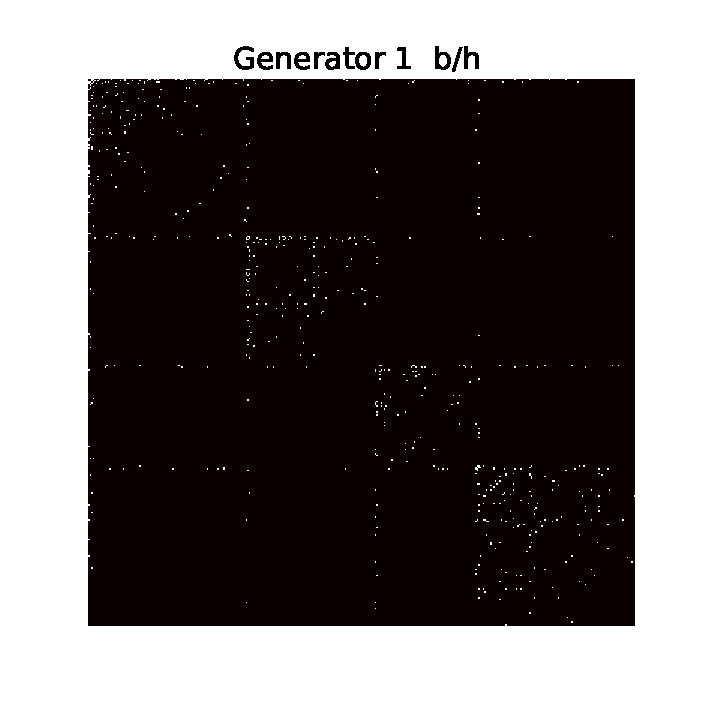
\includegraphics[scale=0.4]{img/g1}
	\endminipage
	\minipage{0.25\textwidth}
	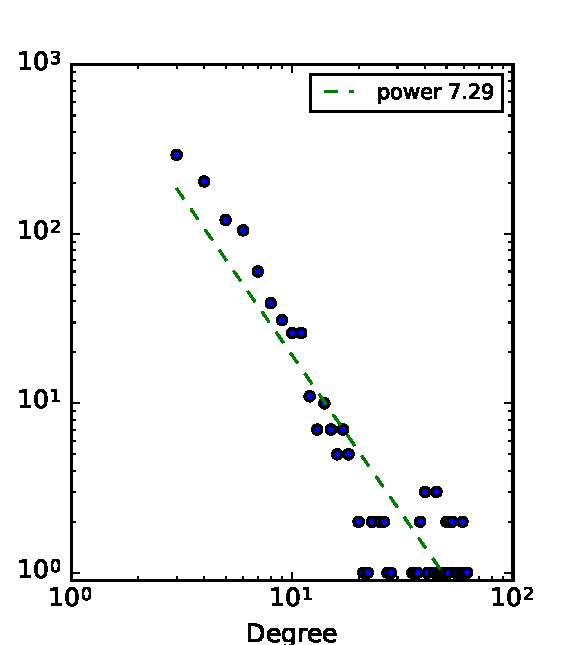
\includegraphics[scale=0.4]{img/g1_d}
	\endminipage
	\vspace{-0.4cm}
	\minipage{0.25\textwidth}
	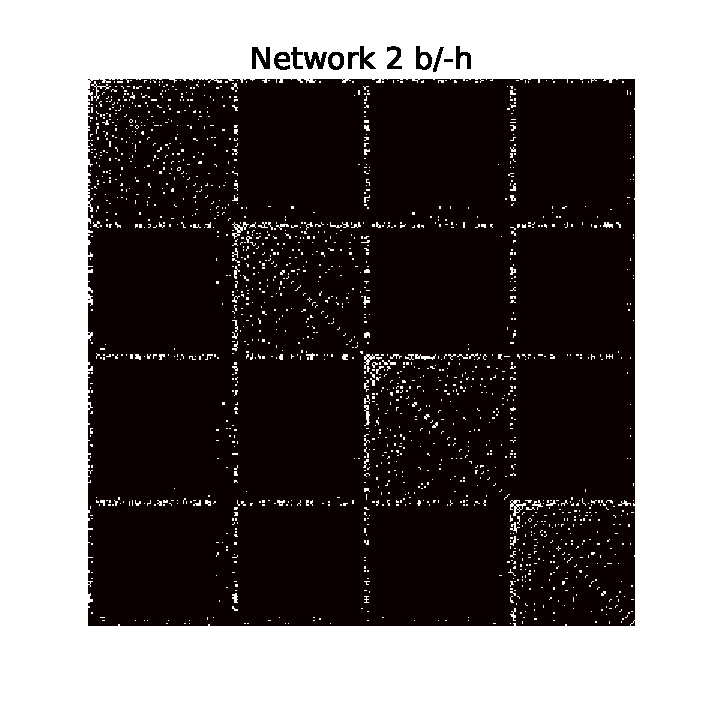
\includegraphics[scale=0.4]{img/g2}
	\endminipage
	\minipage{0.25\textwidth}
	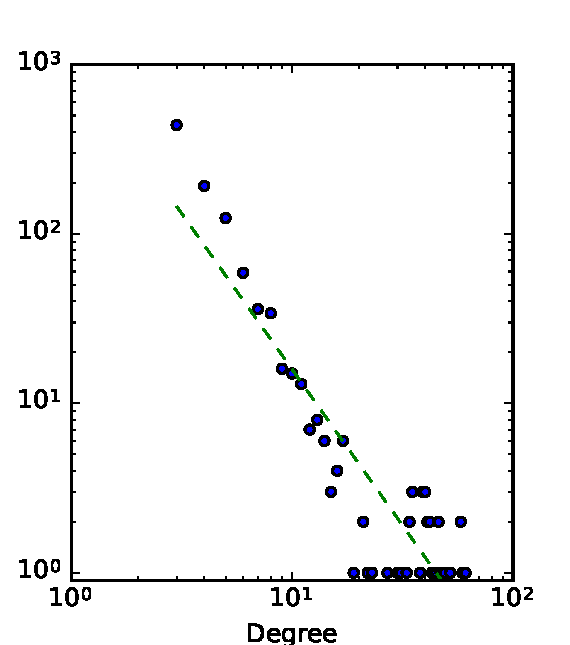
\includegraphics[scale=0.4]{img/g2_d}
	\endminipage
	\vspace{-0.4cm}
	\minipage{0.25\textwidth}
	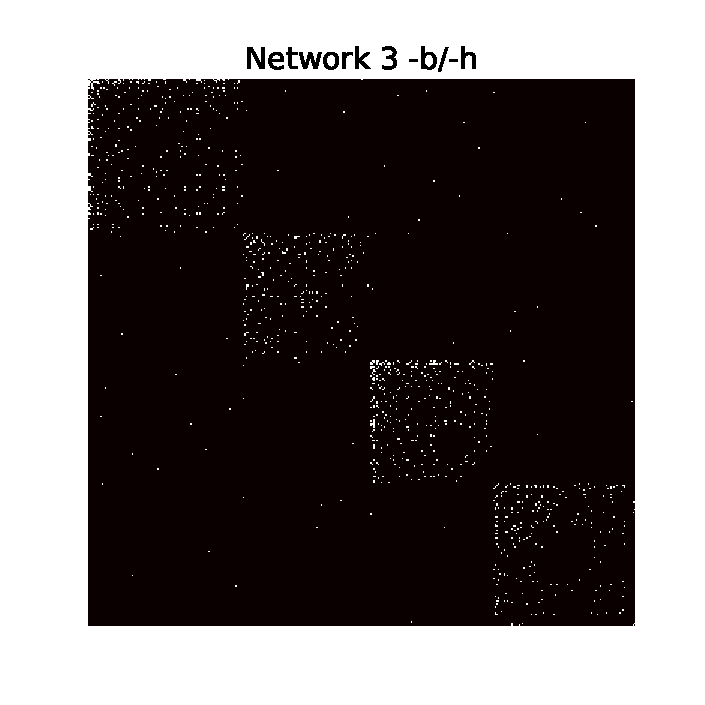
\includegraphics[scale=0.4]{img/g3}
	\endminipage
	\minipage{0.25\textwidth}
	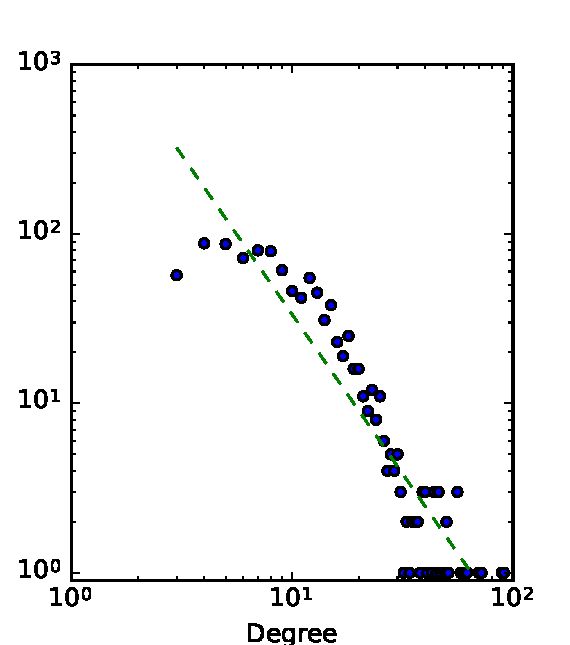
\includegraphics[scale=0.4]{img/g3_d}
	\endminipage
	\vspace{-0.4cm}
	\minipage{0.25\textwidth}
	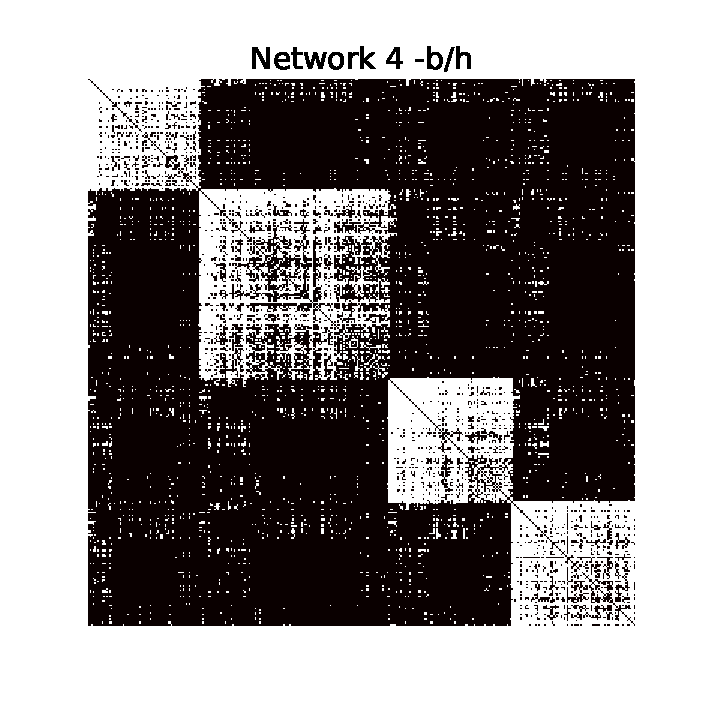
\includegraphics[scale=0.4]{img/g4}
	\endminipage
	\minipage{0.25\textwidth}
	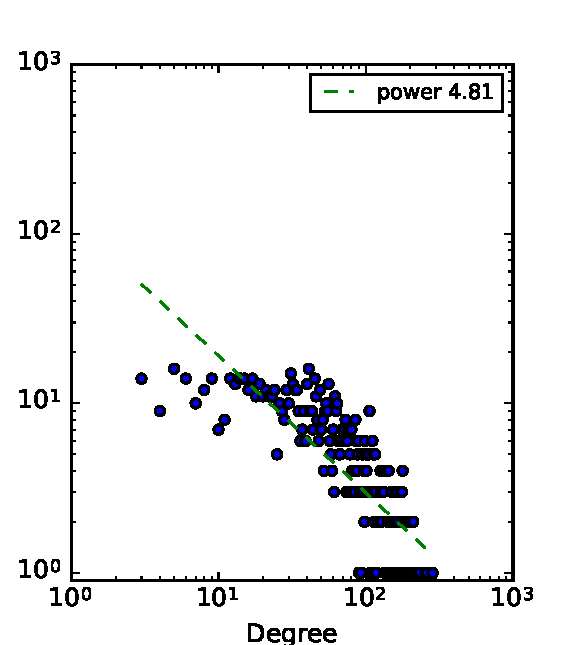
\includegraphics[scale=0.4]{img/g4_d}
	\endminipage
	
	\caption{Left figures represent the adjacency matrices (left) for each of the 4 synthetic networks that we used for the prediction evaluation along their respective global degree distribution in the right plots.}
	\label{fig:synt_graph}
\end{figure}

\begin{figure}[h]
	\centering
	
	
	\minipage{0.25\textwidth}
	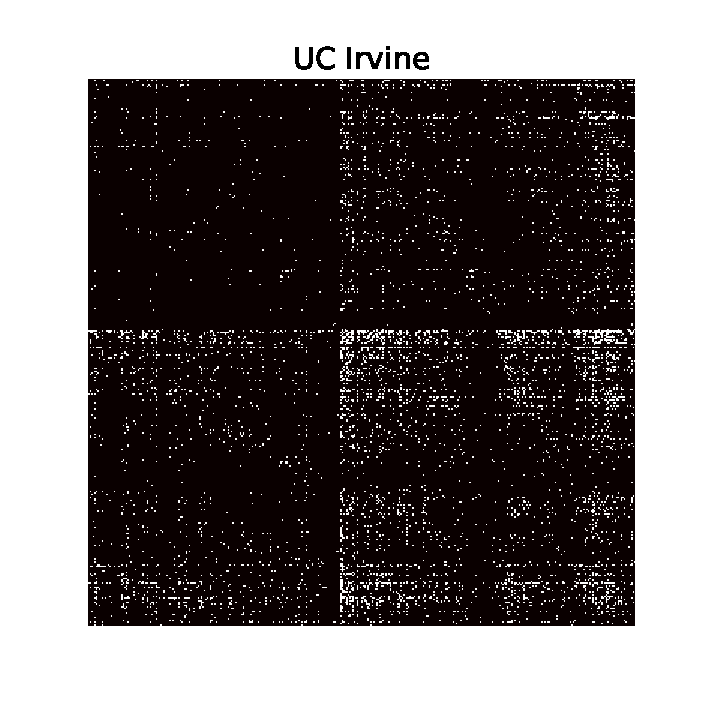
\includegraphics[scale=0.4]{img/irvine}
	\endminipage
	\minipage{0.25\textwidth}
	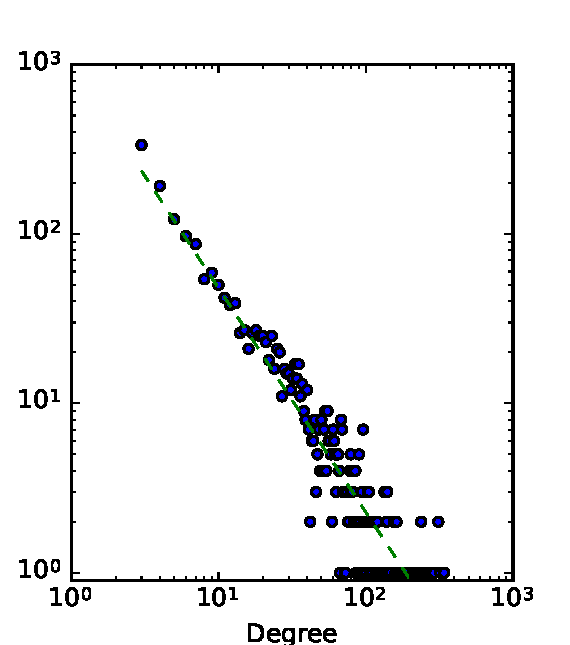
\includegraphics[scale=0.4]{img/irvine_d}
	\endminipage
	\vspace{-0.4cm}
	\minipage{0.25\textwidth}
	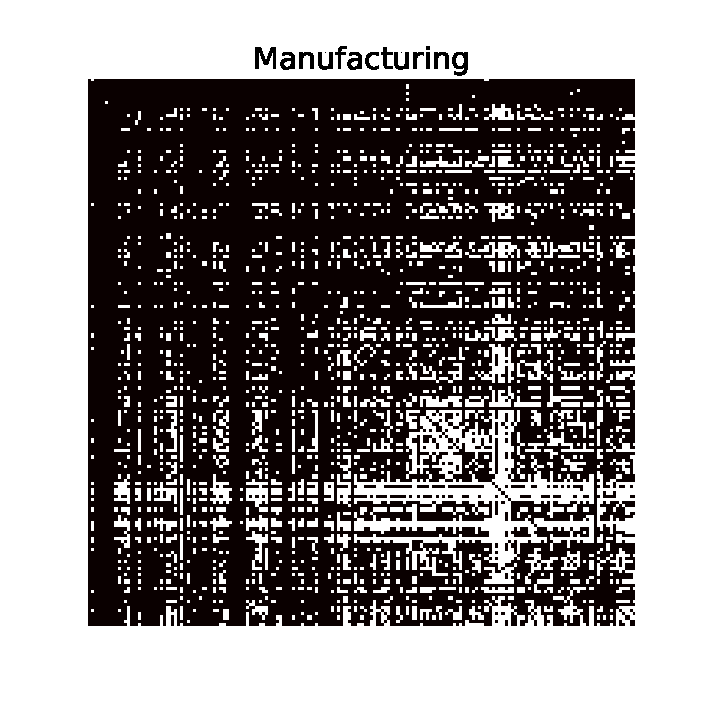
\includegraphics[scale=0.4]{img/manufacturing}
	\endminipage
	\minipage{0.25\textwidth}
	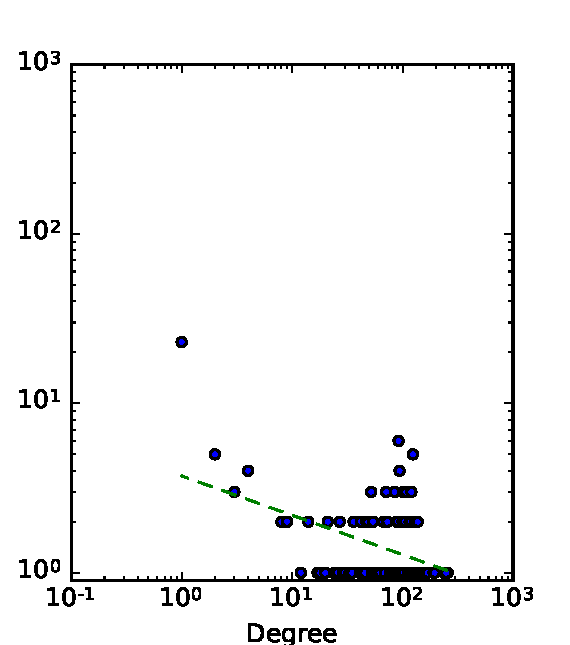
\includegraphics[scale=0.4]{img/manufacturing_d}
	\endminipage
	\caption{Left figures represent the adjacency matrices (left) for each of the 2 real networks that we used for the prediction evaluation along their respective global degree distribution in the right plots.}
	\label{fig:real_graph}
\end{figure}



\subsection{Experimental Settings}
For each datasets described,  we run a MCMC inference consisting of 200 iterations to learn the posterior distribution of each the IMMSB model and ILFM, described in \ref{sec:models}. For IMMSB, concentration parameters of HDP were optimized following \cite{HDP} using vague gamma priors $\alpha_0 \sim \text{Gamma}(1,1)$ and       $\gamma \sim \text{Gamma}(1,1)$. The parameter for the matrix weights were fixed to $\lambda_0=\lambda_1=0.1$. For ILFM, the IBP hyper-parameter was fixed to   $\alpha=0.5$ and the weights hyper-parameter to $\sigma_w = 1$. Each experiences were averaged on 10 repetitions, and results were found to be stable regarding on the random  initialization and the stochastic optimization procedure. 
 

We evaluate the  prediction performance of the models by building a training set and a testing set from the original datasets. In order to achieve this, we build a random mask consisting of 20 percent of the size of the adjacency matrix. This mask is used a our testing set, while the 80 remaining percent are used as a training set.

The inference procedure was run under this settings in all of the 4 synthetic datasets and 2 real networks.

All our experimental platform is available online \footnote{https://github.com/dtrckd/pymake}. It is an ongoing development in order to provide a flexible way to design and run experiments and make data analysis.


\begin{figure}[h]
	\centering
	
	\minipage{0.25\textwidth}
	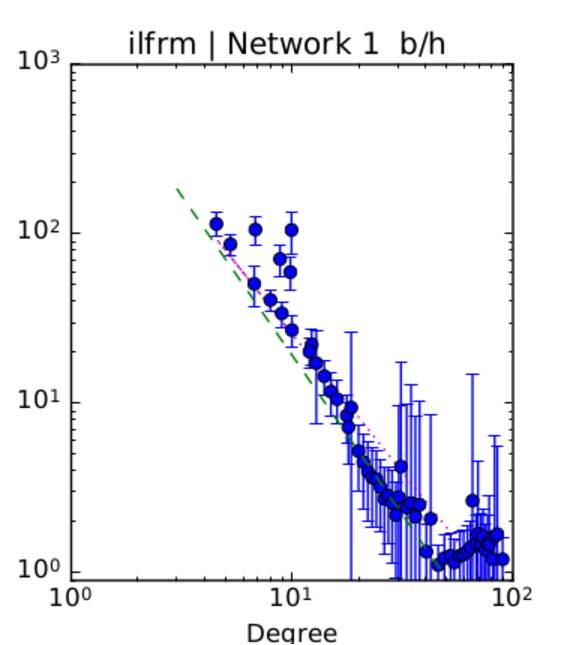
\includegraphics[scale=0.4]{img/ilfrm_g1_d}
	\endminipage
	\minipage{0.25\textwidth}
	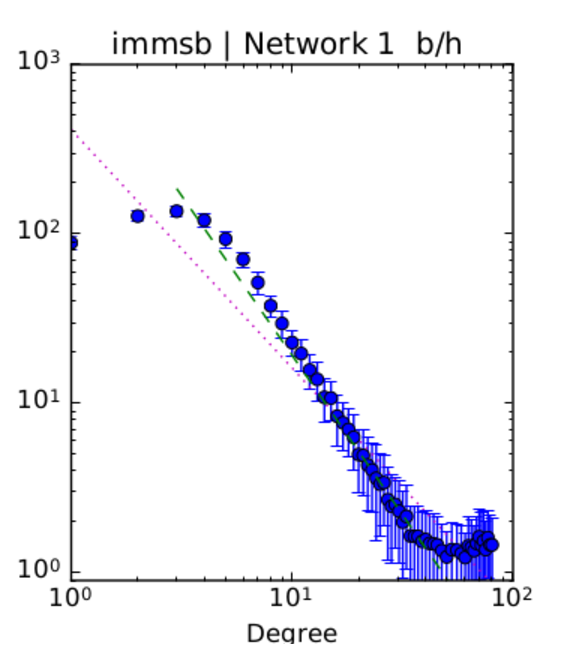
\includegraphics[scale=0.4]{img/immsb_g1_d}
	\endminipage
	\vspace{-0.4cm}
	\minipage{0.25\textwidth}
	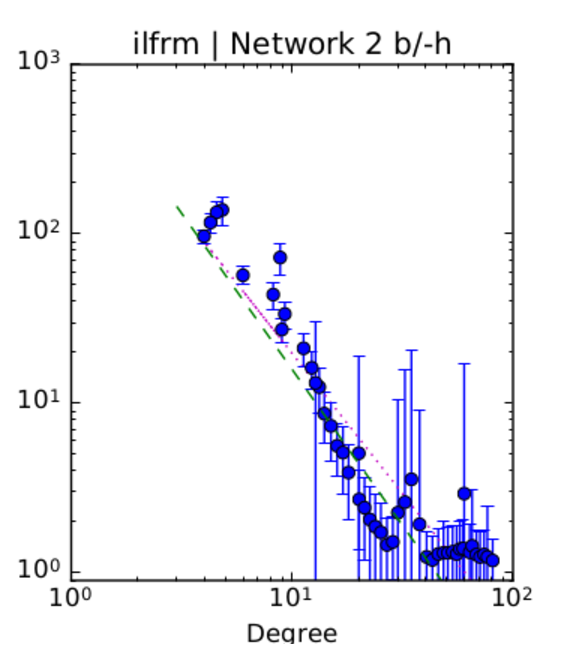
\includegraphics[scale=0.4]{img/ilfrm_g2_d}
	\endminipage
	\minipage{0.25\textwidth}
	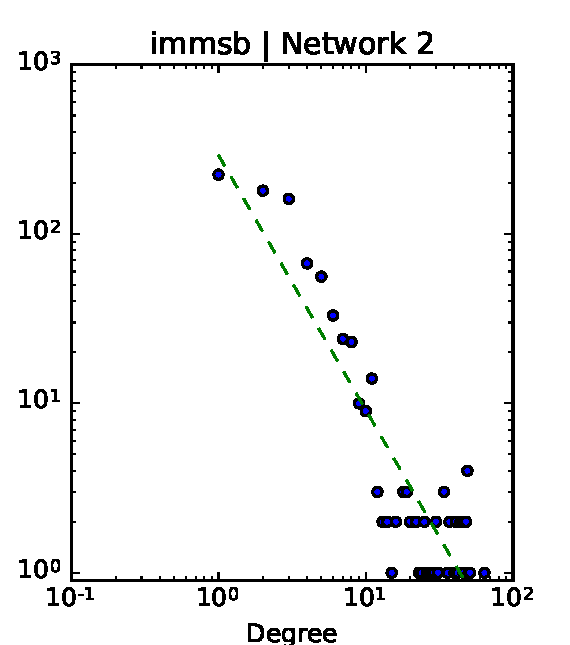
\includegraphics[scale=0.4]{img/immsb_g2_d}
	\endminipage
	\vspace{-0.4cm}
	\minipage{0.25\textwidth}
	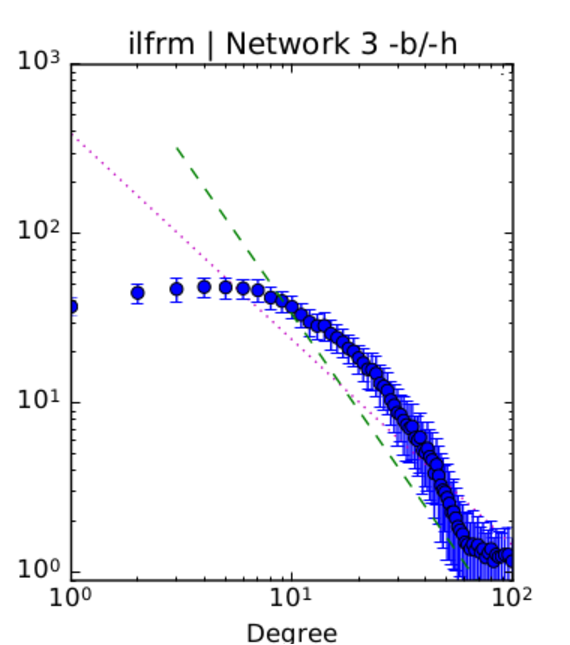
\includegraphics[scale=0.4]{img/ilfrm_g3_d}
	\endminipage
	\minipage{0.25\textwidth}
	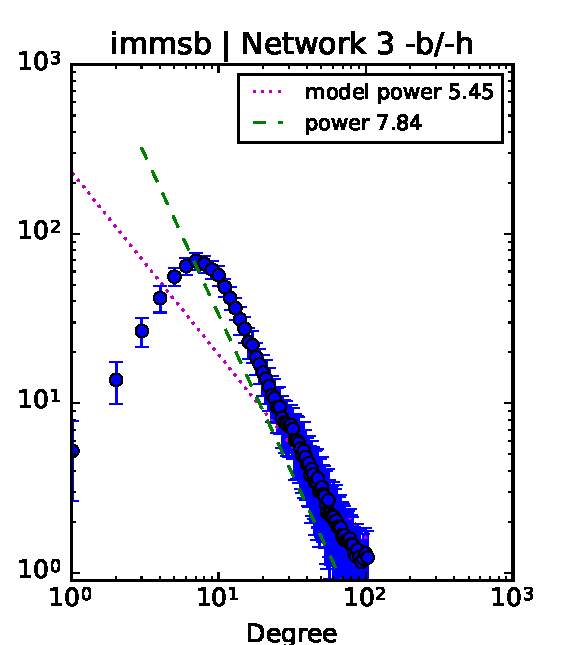
\includegraphics[scale=0.4]{img/immsb_g3_d}
	\endminipage
	\vspace{-0.4cm}
	\minipage{0.25\textwidth}
	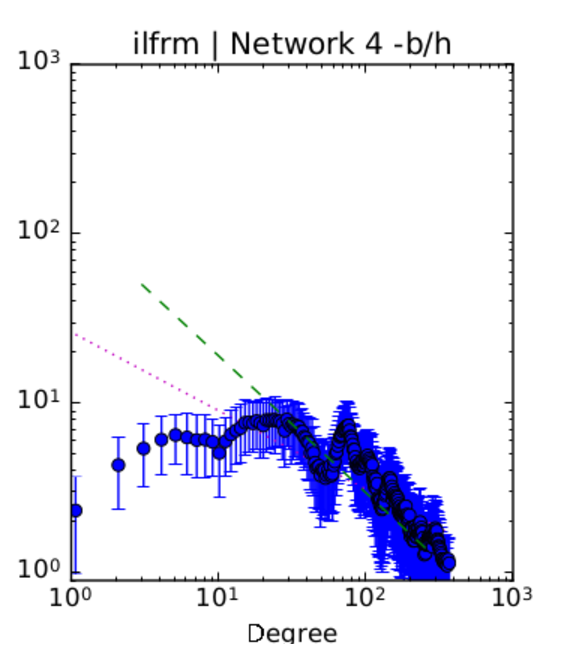
\includegraphics[scale=0.4]{img/ilfrm_g4_d}
	\endminipage
	\minipage{0.25\textwidth}
	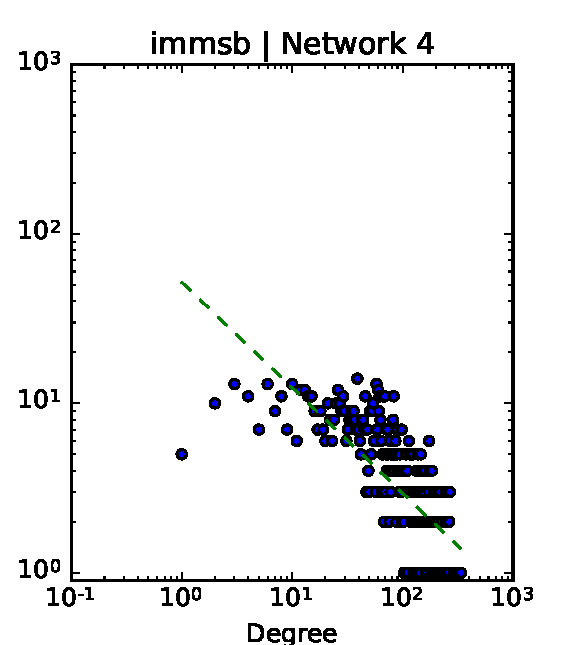
\includegraphics[scale=0.4]{img/immsb_g4_d}
	\endminipage
	
	\caption{Right column is associated to IMMSB and left column to ILFM. Each row is associated to a synthetic networks on which we run the inference procedure. Each figures represent the global degrees distribution for a set of 100 generated networks by the models after its parameters where learned in the corresponding settings.  We also report on these figures two straight lines corresponding of the regression on the degree distribution of the model generated network (dotted) and the regression of the original distribution (dashed) as a qualitative reference.}
	\label{fig:gen_graph_s}
\end{figure}

\begin{figure}[h]
	\centering
	
	\minipage{0.25\textwidth}
	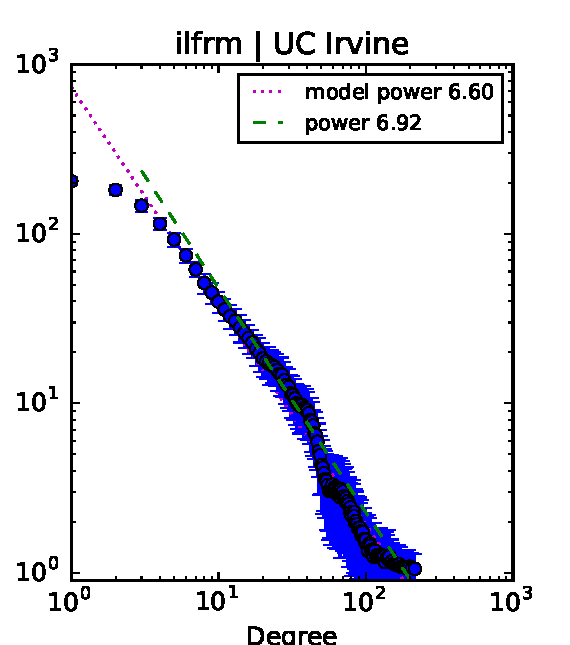
\includegraphics[scale=0.4]{img/ilfrm_irvine_d}
	\endminipage
	\minipage{0.25\textwidth}
	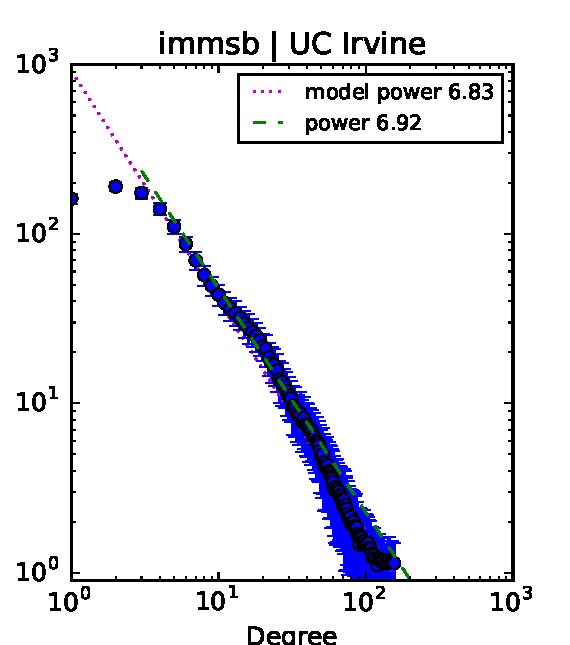
\includegraphics[scale=0.4]{img/immsb_irvine_d}
	\endminipage
	\vspace{-0.4cm}
	\minipage{0.25\textwidth}
	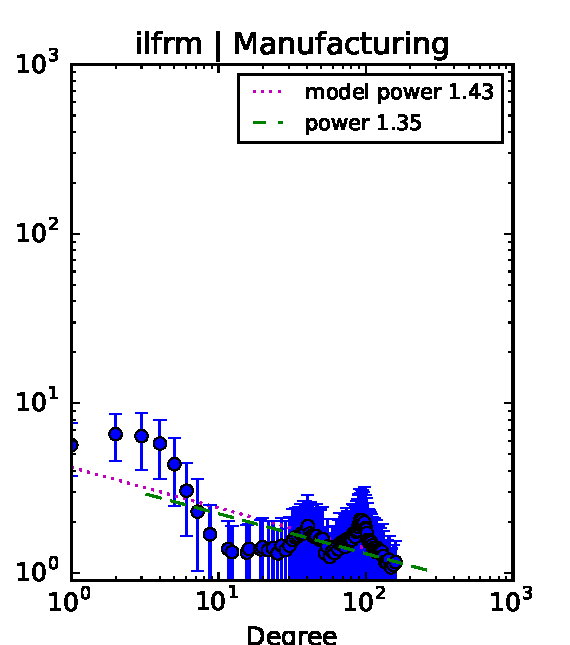
\includegraphics[scale=0.4]{img/ilfrm_manufacturing_d}
	\endminipage
	\minipage{0.25\textwidth}
	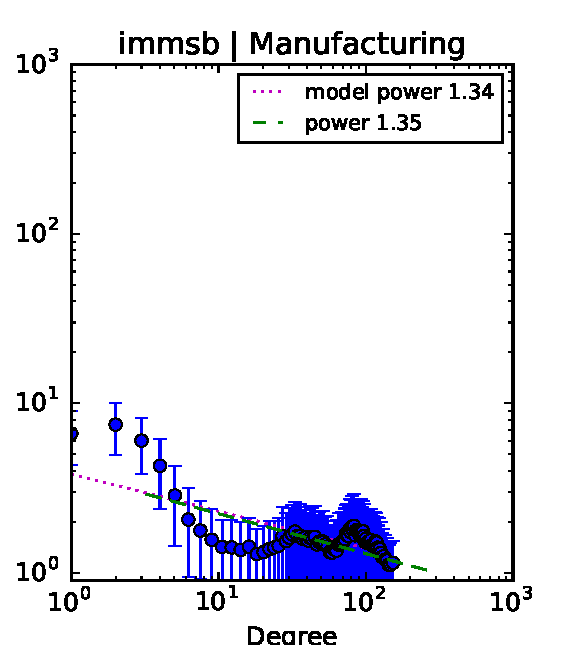
\includegraphics[scale=0.4]{img/immsb_manufacturing_d}
	\endminipage
	
	\caption{Right column is associated to IMMSB and left column to ILFM. Each row is associated to a real networks on which we run the inference procedure. Each figures represent the global degrees distribution for a set of 100 generated networks by the models after its parameters where learned in the corresponding settings. We also report on these figures two straight lines corresponding of the regression on the degree distribution of the model generated network (dotted) and the regression of the original distribution (dashed) as qualitative reference.}
	\label{fig:gen_graph_r}
\end{figure}


\begin{figure}[h]
	\centering
	
	\minipage{0.25\textwidth}
	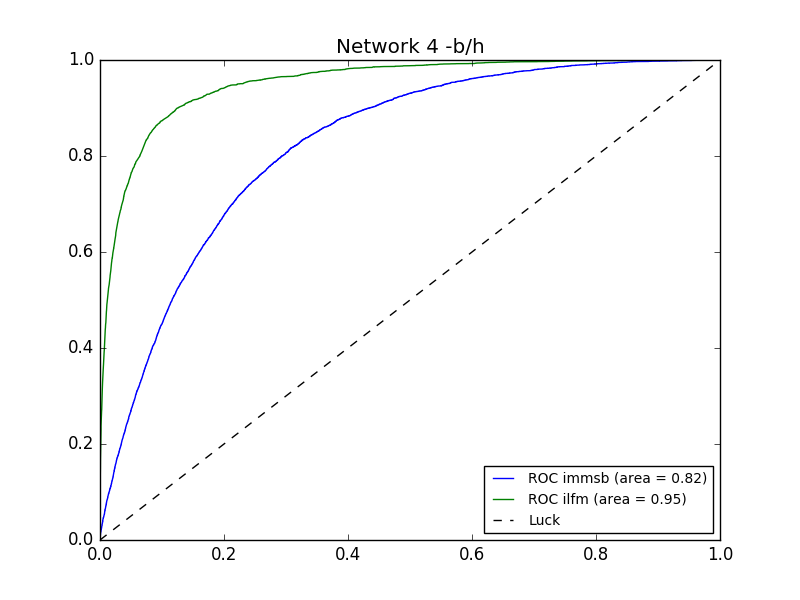
\includegraphics[scale=0.22]{img/M_e/AUC-ROC/figure_1}
	\endminipage
	\minipage{0.25\textwidth}
	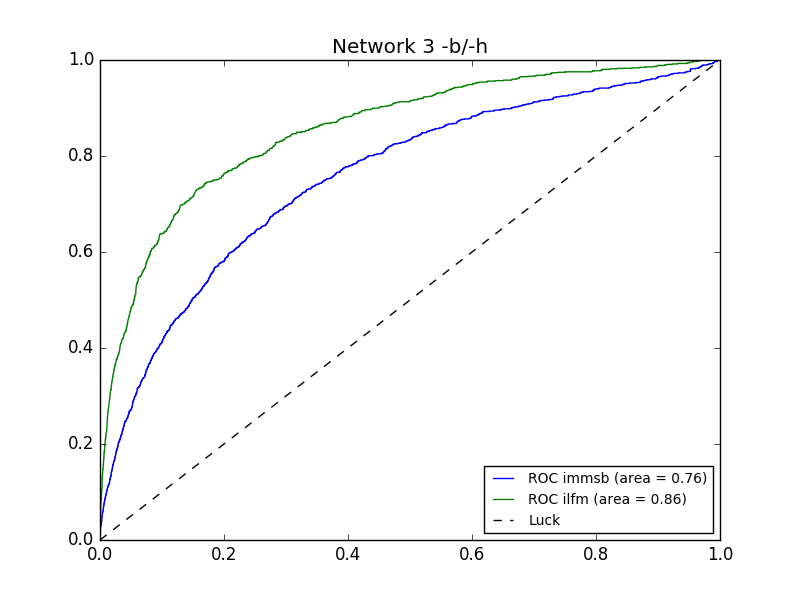
\includegraphics[scale=0.22]{img/M_e/AUC-ROC/figure_2}
	\endminipage
	\vspace{-0.4cm}
	\minipage{0.25\textwidth}
	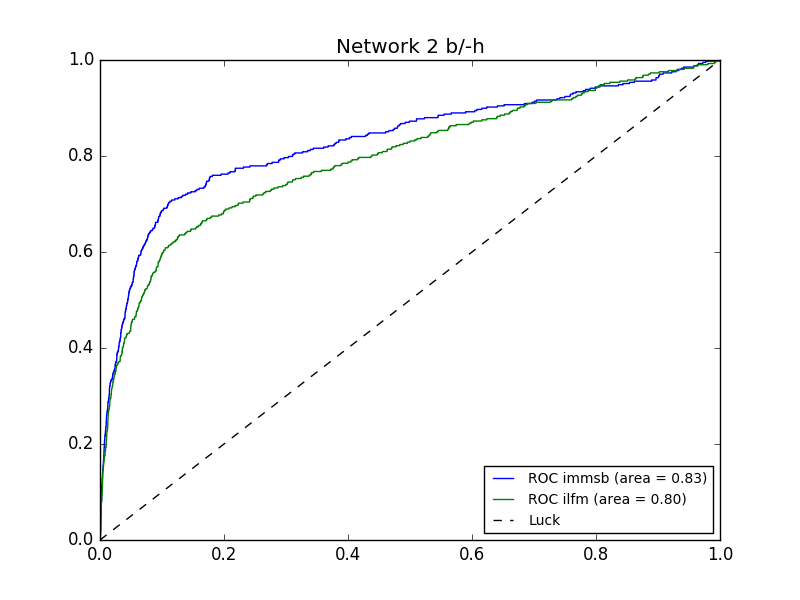
\includegraphics[scale=0.22]{img/M_e/AUC-ROC/figure_3}
	\endminipage
	\minipage{0.25\textwidth}
	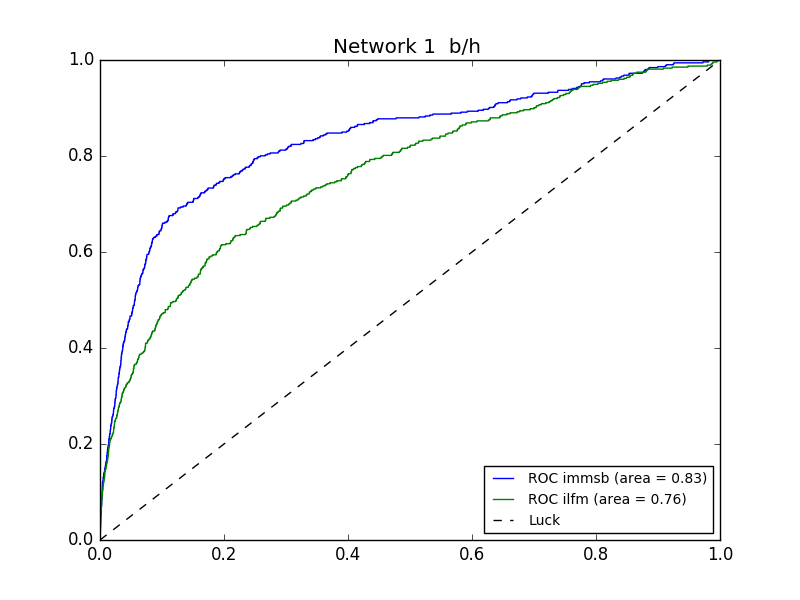
\includegraphics[scale=0.22]{img/M_e/AUC-ROC/figure_4}
	\endminipage
		\vspace{-0.4cm}
	\minipage{0.25\textwidth}
	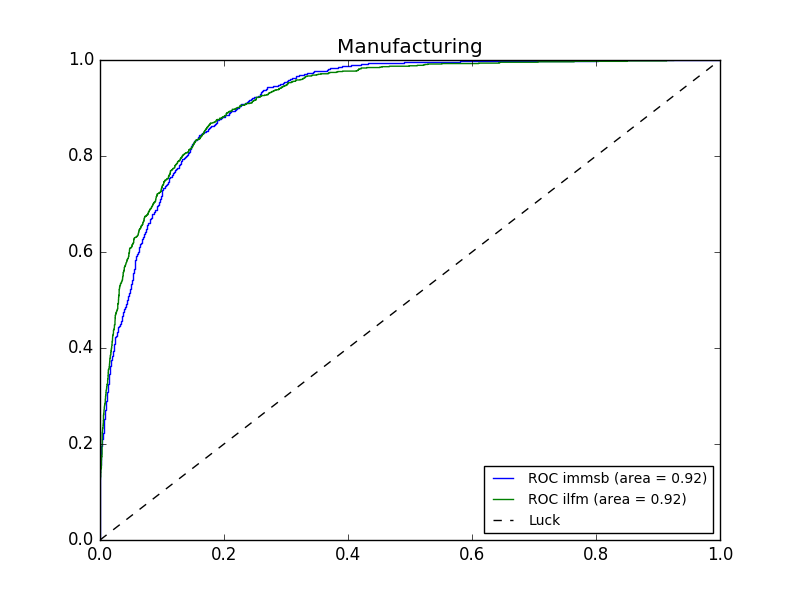
\includegraphics[scale=0.22]{img/M_e/AUC-ROC/figure_5}
	\endminipage
	\minipage{0.25\textwidth}
	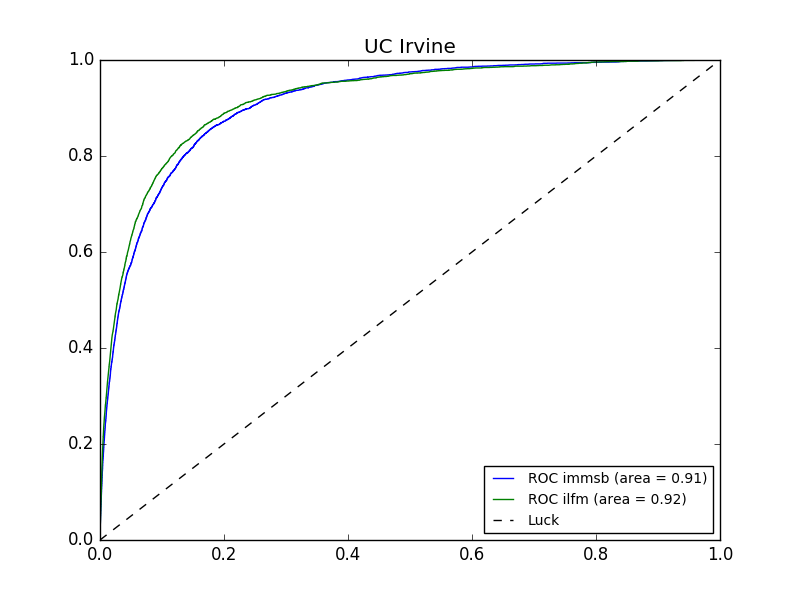
\includegraphics[scale=0.22]{img/M_e/AUC-ROC/figure_6}
	\endminipage
	
	\caption{AUC curves that compare the performance of ILFM and IMMSB on the 4 synthetic networks.}
	\label{fig:auc}
\end{figure}



\subsection{Results}

%%% Figure description:
We report in table \ref{table:unbalanced} our results for the prediction performance in the different settings. The prediction problem is equivalent to a binary prediction problem, where the prediction lies in two classes; edge or not an edge. The local precision and recall in the table concern the links predicted as an edge. The global (precision) refer to the accuracy of the model. The table summarize the precision and recall into the $f_1$ measure. Note that each group of row is indexed by  a number $K$ which indicates various values of initialization of the latent feature dimension.

Comparatively, in figure \ref{fig:auc}, we report the Area Under Curve for each datasets where we compare the prediction performance of IMMSB and ILFM on the task of links prediction.

In figure \ref{fig:gen_graph_s} and \ref{fig:gen_graph_r} we used the models learned on the training datasets to generate full networks and report the global degree distribution of such generated networks. 

%%% What the figure tells:
The first thing to note is that comparing the performance between both models in the links prediction precision and recall (ref{table:unbalanced}), can seem to conflict with results in the ROC curve (\ref{fig:auc}). More precisely we see that ILFM dominate IMMSB on the $f_1$ measures on all experiments except for one (network 1, K=15). But on the AUC-ROC analysis( \ref{fig:auc}) we see that IMMSB dominate ILFM for two networks (Networks 1 and Networks 2), although it's number of latent feature is almost half lesser than for ILFM. This behavior is also reflected on the accuracy for both models (global precision); The accuracy of IMMSB models is higher for the Network1 and Network2, and this is the opposite for ILFM, which are more accurate for Network3 and Network4. Interestingly, we see that for ILFM, the dimension of the latent feature for which ILFM converged, for the two first networks is significantly higher than the two other. In other words the ILFM model try to compensate is weak performance by increasing the number of features.

In the other hands, according to the degree distribution of the 4 synthetic networks we fitted, (figure \ref{fig:synt_graph}) and the p-value associated the power law hypothesis (table \ref{table:artificial_networks}), we see that the Network1 and Network2 has a stronger preferential attachment effects than Network3 and Network4.


Finally, the difference of behaviors of the models according to the training networks is captured by the randomness of the (generated) degree distributions (figure \ref{fig:gen_graph_s} ). We see that the degree distribution corresponding to the two bursty synthetic network, has  a high variance for ILFM while it is quite smooth for IMMSB.

The success of ILFM on bursty networks reflects the fact ILFM can handle the local preferential attachments and not ILFM. We assume that this symptom for ILFM is due to the hard assignment of it's latent features, where a difference of one feature, in a feature vector, can lead to a big gap in the probability to generate a link. A phenomenon particularly strong for very bursty networks where the long tail makes the distribution of degrees more sensitive to little change.

\textcolor{red}{Nothing about real networks: result are not really interesting except why ILFM variance of degree distribution on bursty networks fb\_uc is smooth ? }

To conclude, these experiments show that a properties based approach can help to choose an appropriate models. Moreover a model that seems to outperforms an other with a particular measure could be non optimal depending on what we want to capture in the data, keeping in mind that one measures is associated, in some way, to one behaviors or property.
